\section{Einheit}
\label{kap:McpExecutorEinheitMain}
Die Mcp-Executor-Einheit definiert ein Ger�t, welches Beschleunigungsdaten �ber SPI an ein Master-Ger�t schickt, sobald es eingeschaltet wird.
\newline
F�r diese Funktionalit�t werden die in Kapitel \ref{kap:McpExecutorVerwendeteKomponenten} beschriebenen Komponenten verwendet, welche wie in Abbildung \ref{fig:Mcp2515EinheitZusammenspiel} dargestellt entsprechend verkn�pft sind.

	\begin{figure}[H]
		\centering
		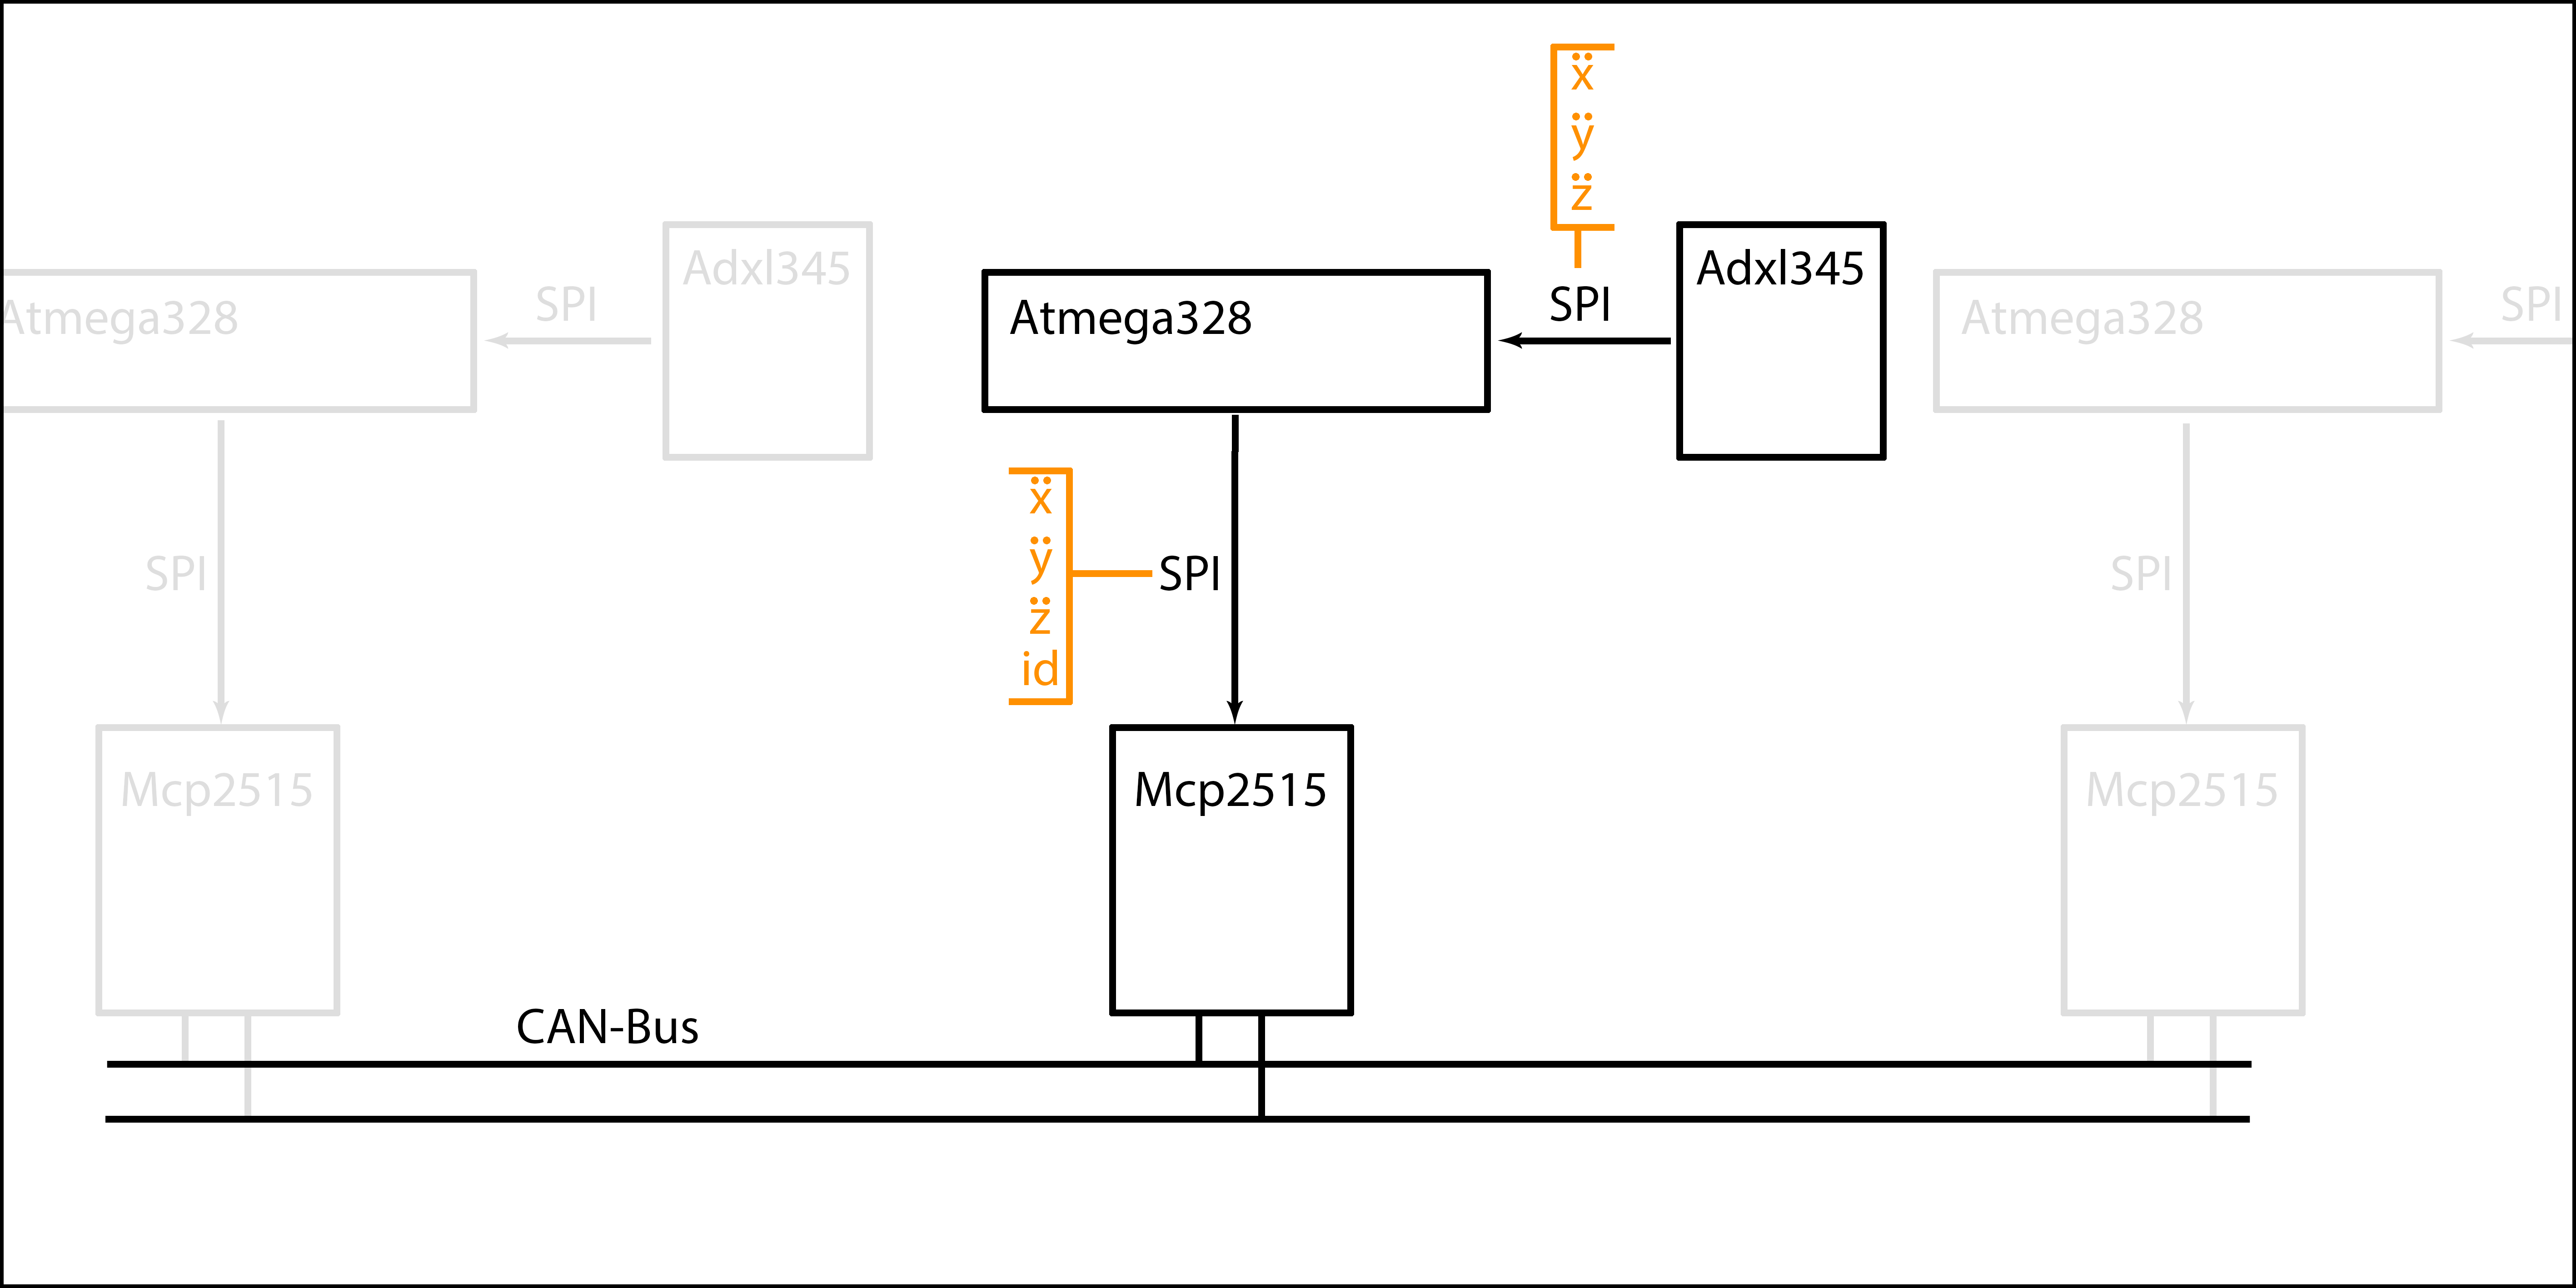
\includegraphics[width=1.0\linewidth]{03_Grafiken/Messsystem/Mcp2515EinheitZusammenspiel}
		\caption[Zusammenspiel der Komponenten Mcp-Executor-Einheit]{Zusammenspiel der Komponenten Mcp-Executor-Einheit}
		\label{fig:Mcp2515EinheitZusammenspiel}
	\end{figure}
	
Der Microcontroller Atmega328 lie�t von dem Beschleunigungssensor Adxl �ber die Schnittstelle SPI Sensordaten aus und gibt diese (ebenfalls �ber SPI) an den Mcp2515 weiter. Dieser schiebt die Daten auf den CAN-Bus.
	
\subsection{Verwendete Komponenten}
\label{kap:McpExecutorVerwendeteKomponenten}
F�r eine Einheit werden verschiedene Hardware-Komponenten verwendet, deren Wahl vor allem hinsichtlich des Kostenaufwandes erfolgte. Auch die Bauteilgr��e ist ein entscheidender Faktor, da die Einheiten m�glichst nicht st�rend sein sollen.

\begin{itemize}
	\item \textbf{Mcp2515}
	
	Der Mcp2515 beschreibt an sich den Chip, welcher auf der, in Abbildung \ref{fig:Mcp2515} dargestellten, Platine verbaut ist. Dieser Name wird jedoch f�r den gesamten Chip verwendet.
	\newline
	Die Funktion des Mcp2515 besteht darin Daten �ber die Schnittstelle SPI zu empfangen und �ber einen CAN-Bus zu versendet. Die Steuerung des Chips (z.B. Beschreiben eines Sende-Buffers) erfolgt dabei mit entsprechenden Kommandos �ber SPI. Das Konvertieren in L-, H-Pegel erfolgt komplett automatisch.
	
	\begin{figure}[H]
		\centering
		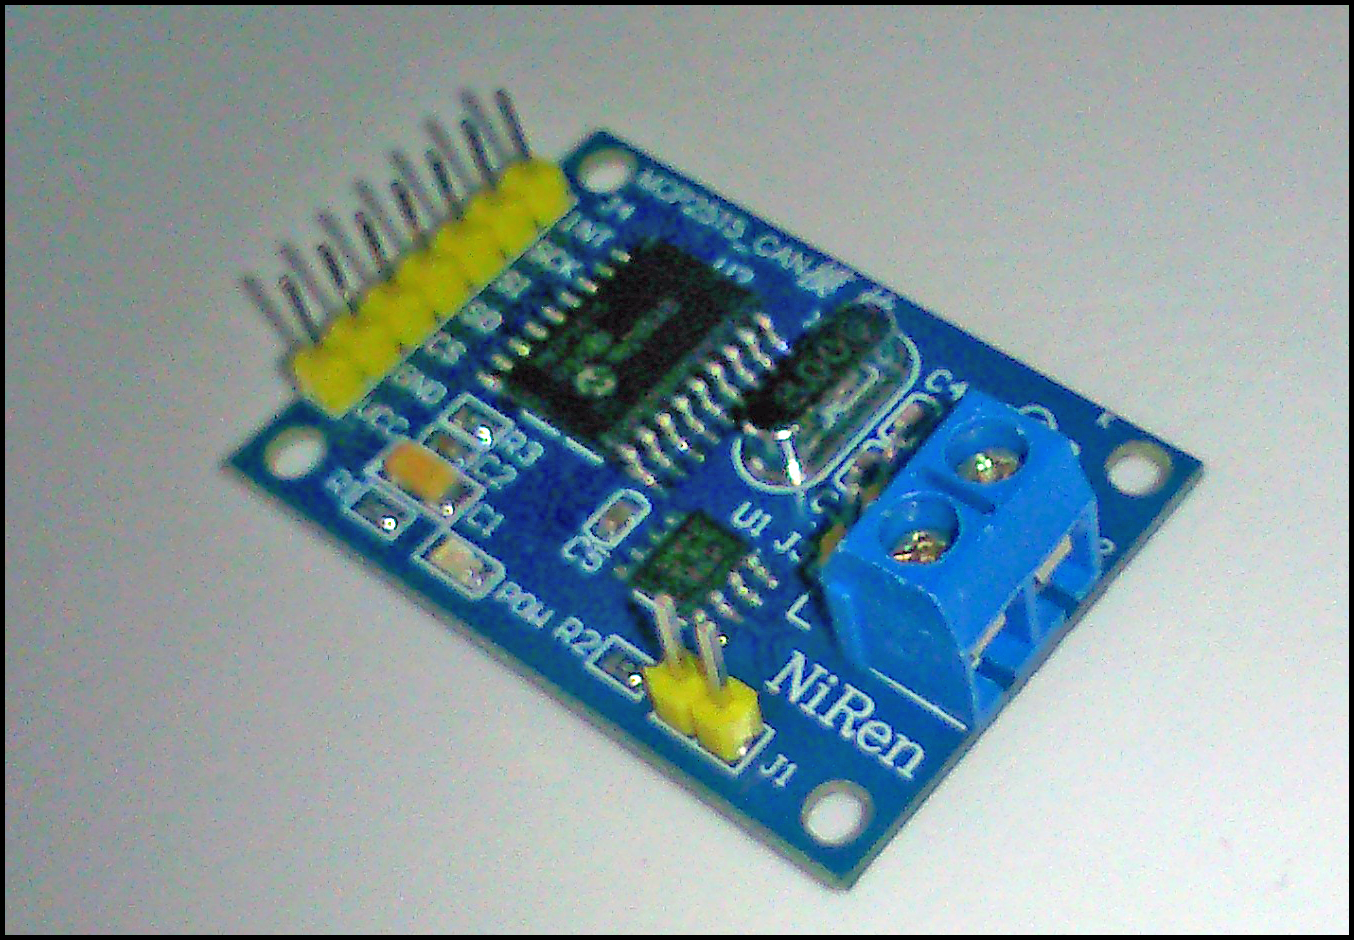
\includegraphics[width=0.4\linewidth]{03_Grafiken/Messsystem/Mcp2515}
		\caption[Mcp2515]{Mcp2515}
		\label{fig:Mcp2515}
	\end{figure}
	
	\item \textbf{Adxl345}
	
	Bei dem Adxl345 handelt es sich um einen 3-Achsen Beschleunigungssensor (s. Abbildung \ref{fig:Adxl345}), dessen Messwerte �ber SPI in verschiedenen Genauigkeiten ausgelesen werden k�nnen.
	Der Chip besitzt eine �u�erst geringe Leistungsaufnahme und ist kompatk in seiner Bauform.
		
	\begin{figure}[H]
		\centering
		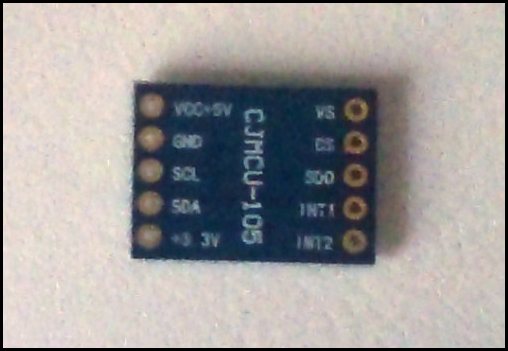
\includegraphics[width=0.4\linewidth]{03_Grafiken/Messsystem/Adxl345}
		\caption[Adxl345]{Adxl345}
		\label{fig:Adxl345}
	\end{figure}
	
	\item \textbf{Atmega328}
	
	Der Microcontroller Atmega328 ist u.A. in dem Arduino-Board verbaut. Es ist ein kostenf�nstiger Allrounder, welcher haupts�chlich wegen seiner gro�en Verbreitung gew�hlt wurde.
	Der Chip (s. Abbildung \ref{fig:Atmega328}) besitzt eine SPI-Schnittstelle und diverse I/O's, weshalb die Projektanforderungen vollst�ndig erf�llt werden.
	\newline
	Es exisiteren zwei verschiedene Versionen des MCU's, von denen die Atmega328-P Variante f�r eine geringe Leistungsaufnahme konzipiert ist. 
	
	\begin{figure}[H]
		\centering
		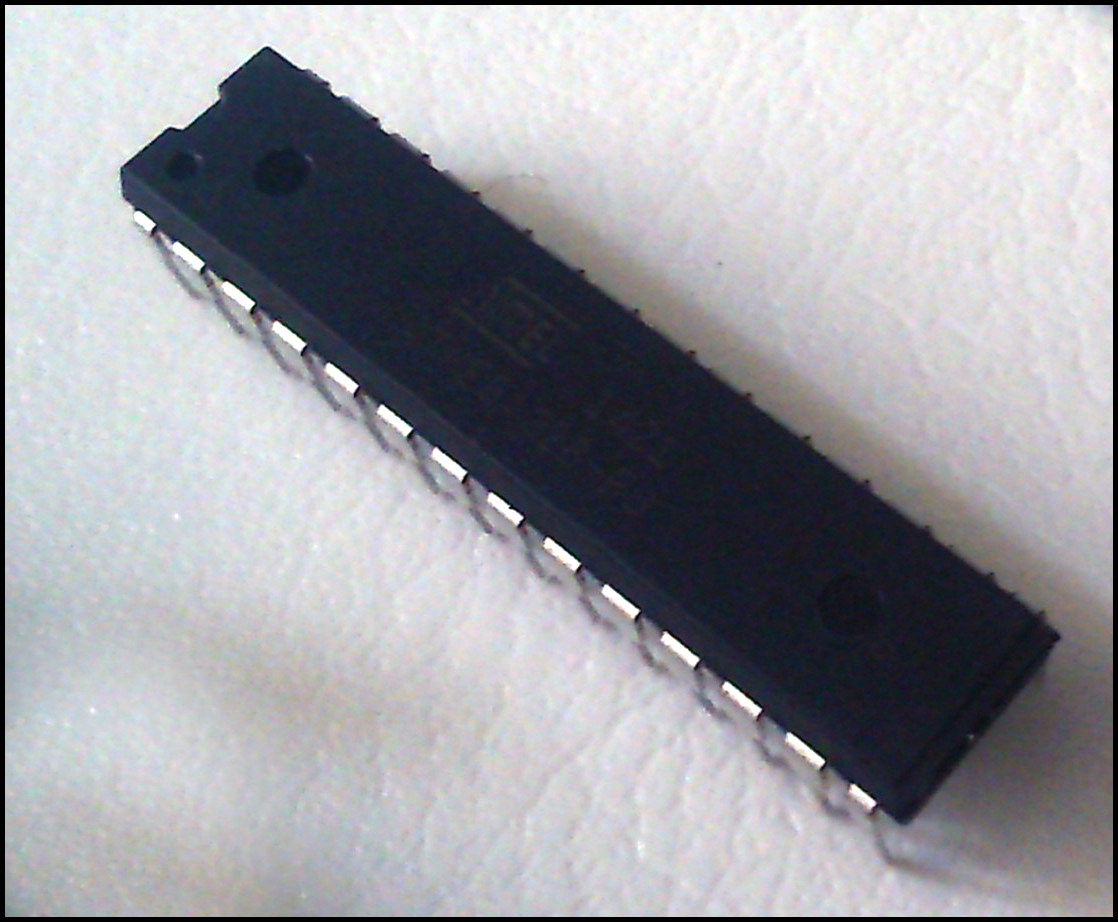
\includegraphics[width=0.4\linewidth]{03_Grafiken/Messsystem/Atmega328}
		\caption[Atmega328]{Atmega328}
		\label{fig:Atmega328}
	\end{figure}
	
	\item \textbf{Oscillator und Kondensator}
	
	Der Atmega328 ben�tigt einen externen Taktgeber, welcher mit einem 16Mhz Quarz und entsprechenden Kondensatoren gew�hlt wird (s. Abbildung \ref{fig:Oscillator}).
	
	\begin{figure}[H]
		\centering
		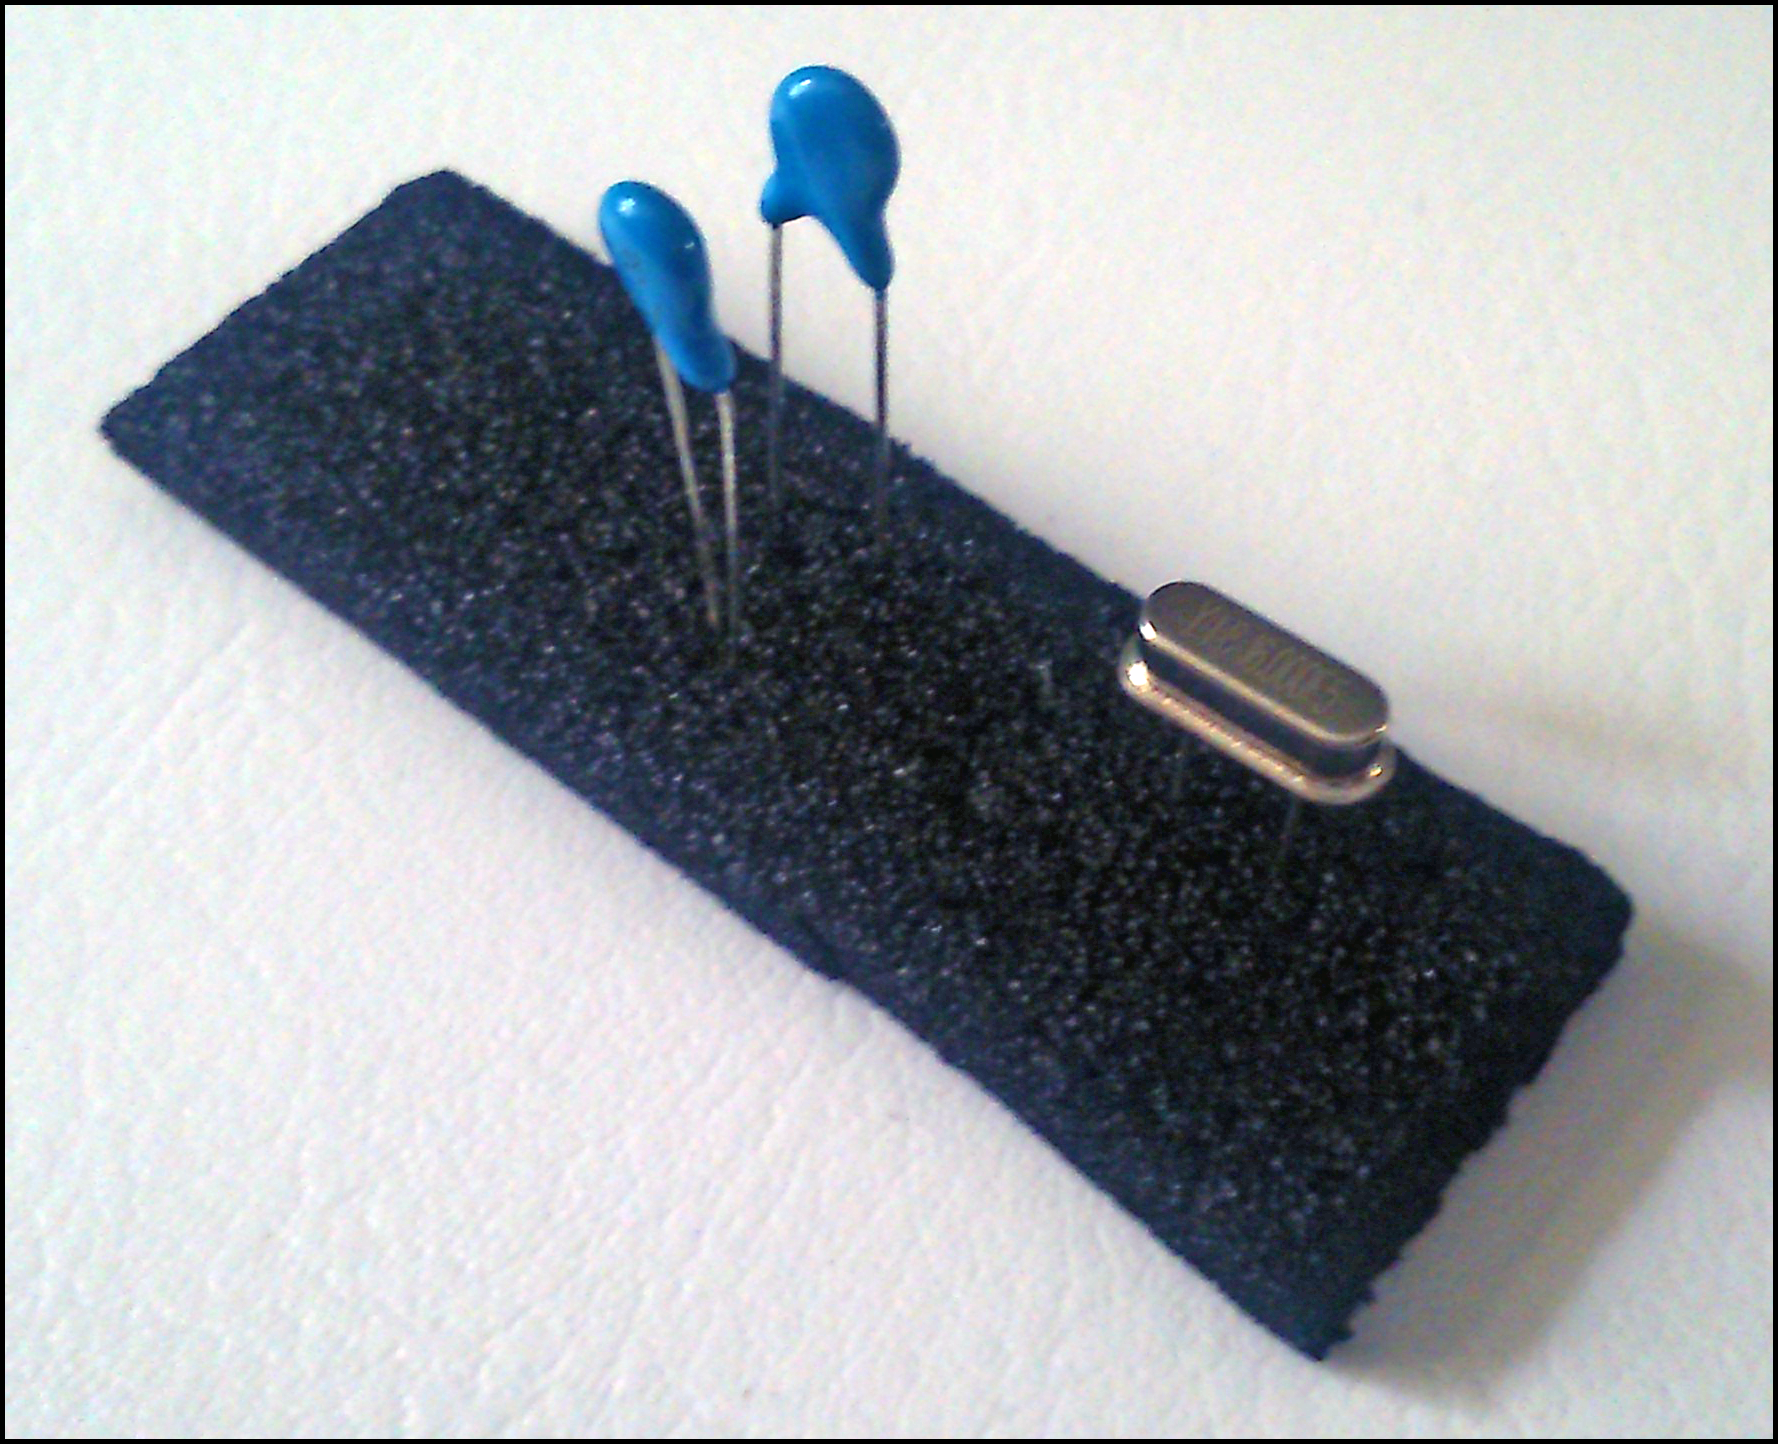
\includegraphics[width=0.4\linewidth]{03_Grafiken/Messsystem/Oscillator}
		\caption[Oscillator]{Oscillator}
		\label{fig:Oscillator}
	\end{figure}
		
\end{itemize}
\subsection{Testversion}
\label{kap:McpExecutorTestversion}
Um die Funktionen der Chips zu verstehen und beherrschen zu k�nnen erfolgt der Aufbau einer Einheit auf einem Entwicklungsboard (Whiteboard). Dieser Aufbau beinhaltet alles, was f�r eine Einheit vorgesehen ist, d.h. einen Atmega328 (mit externem Taktgeber), einen Adxl345 und einen Mcp2515. Mit entsprechender Verdrahtung (s. Schaltbild \ref{fig:SchaltbildEinheit}) und der Entwicklung eines Programms, welches auf der MCU aktiv ist, lassen sich die Sensorwerte �ber einen CAN-Bus auslesen. Die Sensor-ID muss programmatisch auf der MCU definiert werden. 

\begin{figure}[H]
	\centering
	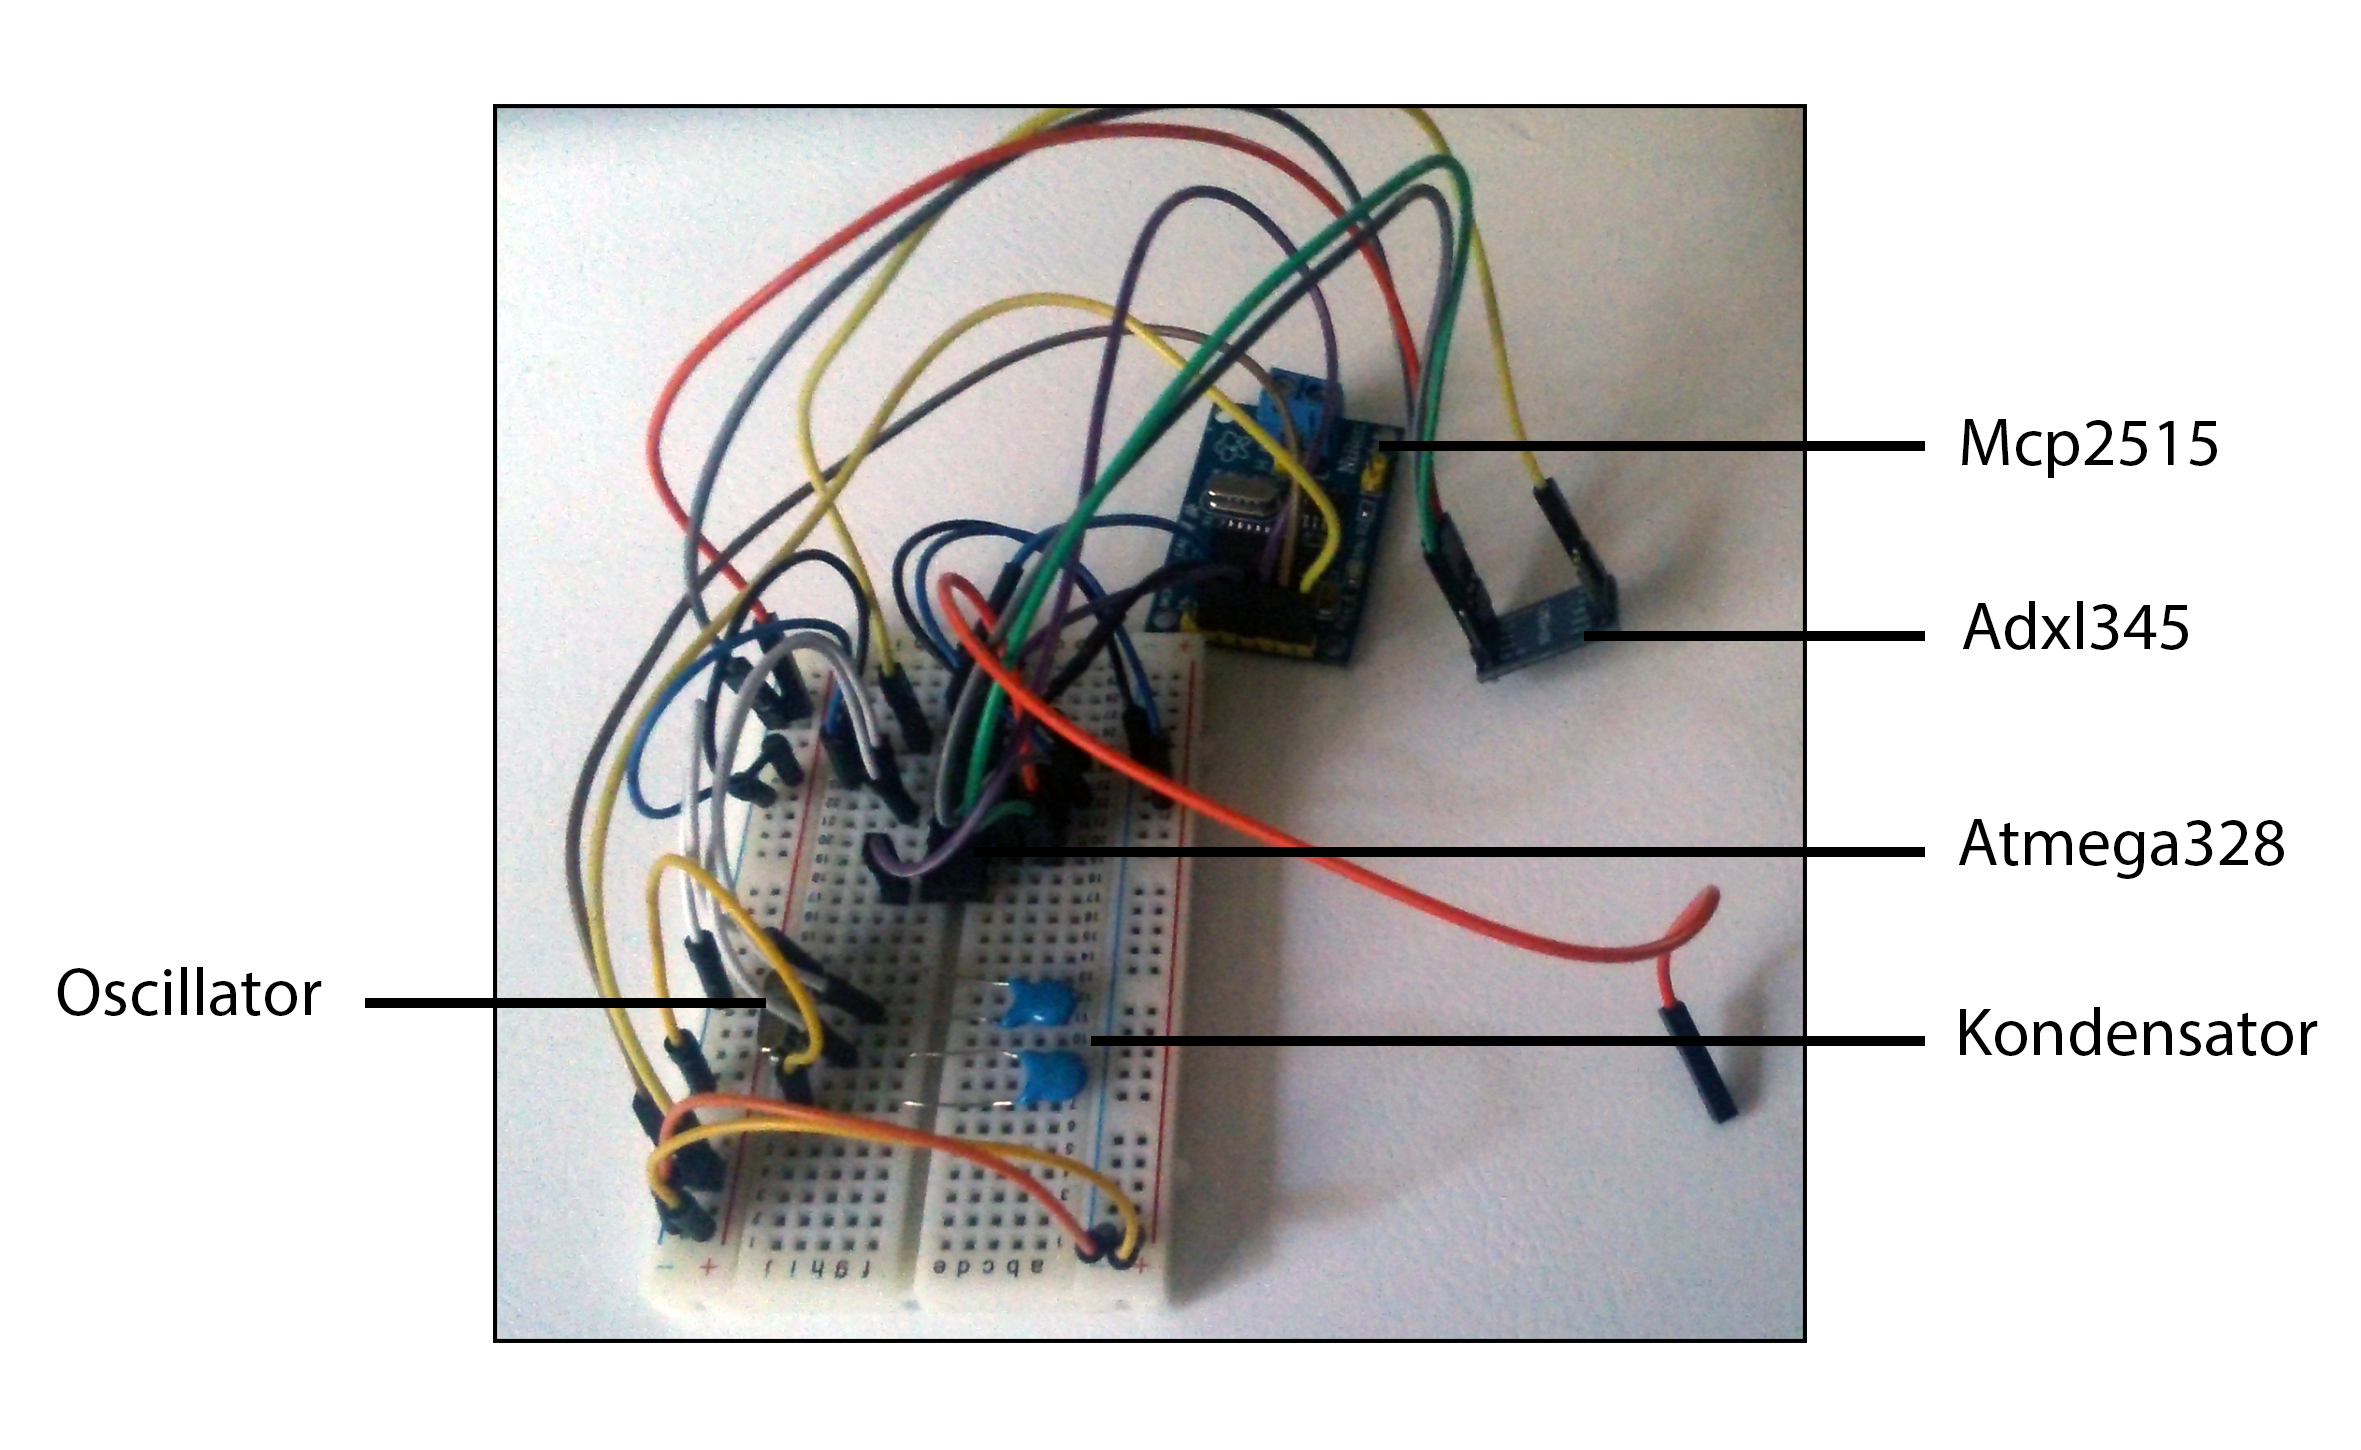
\includegraphics[width=0.9\linewidth]{03_Grafiken/Messsystem/McpExecutorTest}
	\caption[Testversion einer Mcp-Executor-Einheit]{Testversion einer Mcp-Executor-Einheit}
	\label{fig:McpExecutorTest}
\end{figure}

Mit zwei solcher Testaufbauten wurde das Aufnehmen von Sensorwerten validiert.
\subsection{Beta version}
\label{kap:McpExecutorBetaversion}
F�r die Betaversion der Mcp-Executor-Einheit werden alle Komponenten in ein Geh�use integriert (s. Abbildung \ref{fig:McpExecutorBeta}), welches gerade so gro� ist, dass es beim Tragen am K�rper m�glichst nicht st�rt und einfach befestigt werden kann. F�r das Integrieren werden zus�tliche Platinen angefertigt.
\newline
Aufgrund des Feststellens verschiedener negativer Aspekte w�hrend der Entstehung der Einheiten existieren mehrere Beta-Versionen, von denen jedoch nur die erste aufgeziegt wird.

\begin{figure}[H]
	\centering
	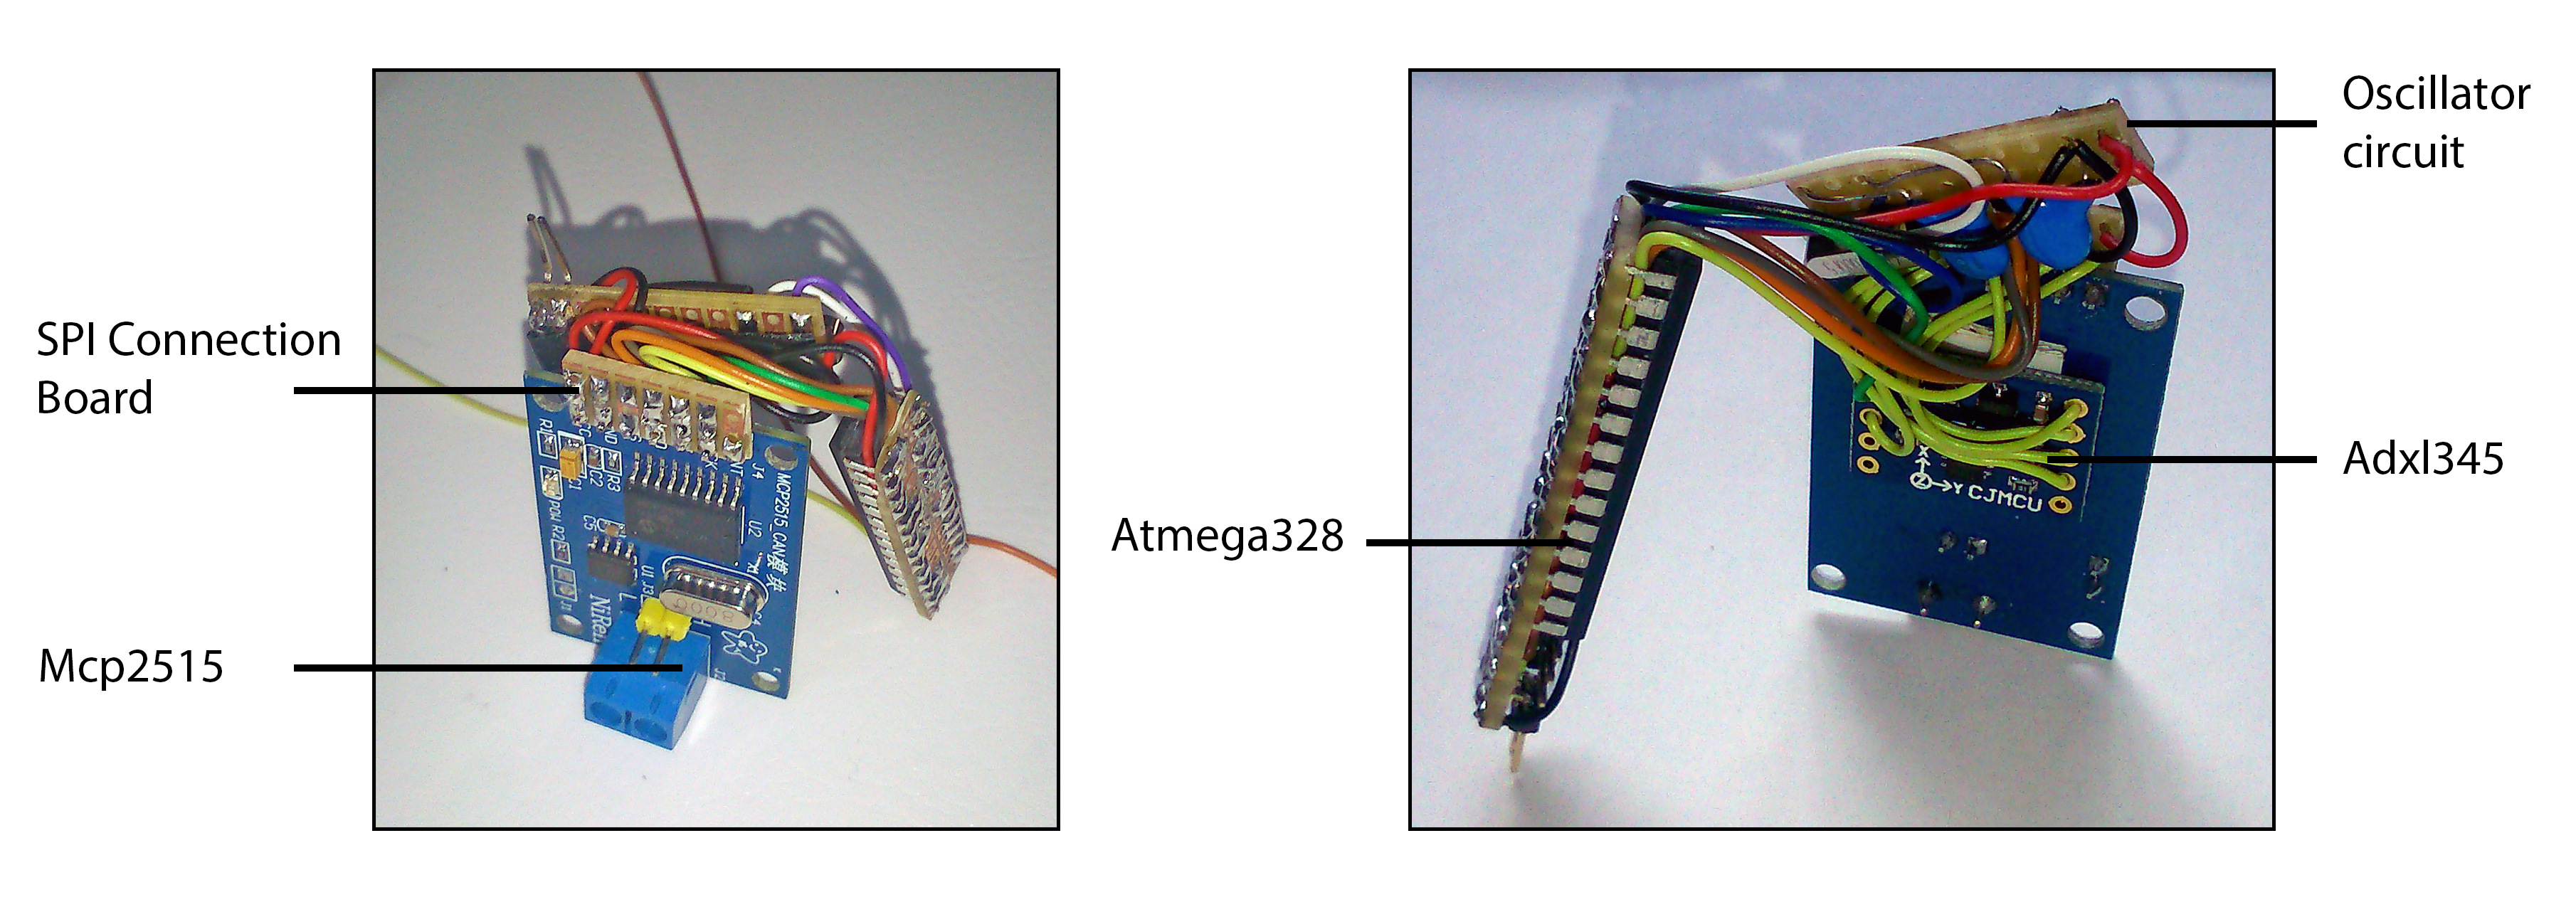
\includegraphics[width=1.0\linewidth]{03_Grafiken/Messsystem/McpExecutor_BetaDetail}
	\caption[Betaversion einer Mcp-Executor-Einheit]{Betaversion einer Mcp-Executor-Einheit}
	\label{fig:McpExecutorBeta}
\end{figure}

Die Befestigung der Einheit am K�rper erfolgt anhand eines Positioniergurtes. Dieser besteht in der ersten Beta-Version aus zwei und Klettverschl�ssen, die an dem Abdeckblech der Einheit befestigt sind. Durch ein entsprechendes Gegenst�ck des Klettverschlusses auf der R�ckseite des Abdeckblechs ist der notwendige Halt gegeben.\\
An dem Anzug sind ebenfalls entsprechende Gegenst�cke des Klettverschlusses angebracht, sodass die Einheiten w�hrend der Bewegung nicht verrutschen. 

%
% BILD KLETTVERSCHLUSS
%
\begin{figure}[H]
	\centering
	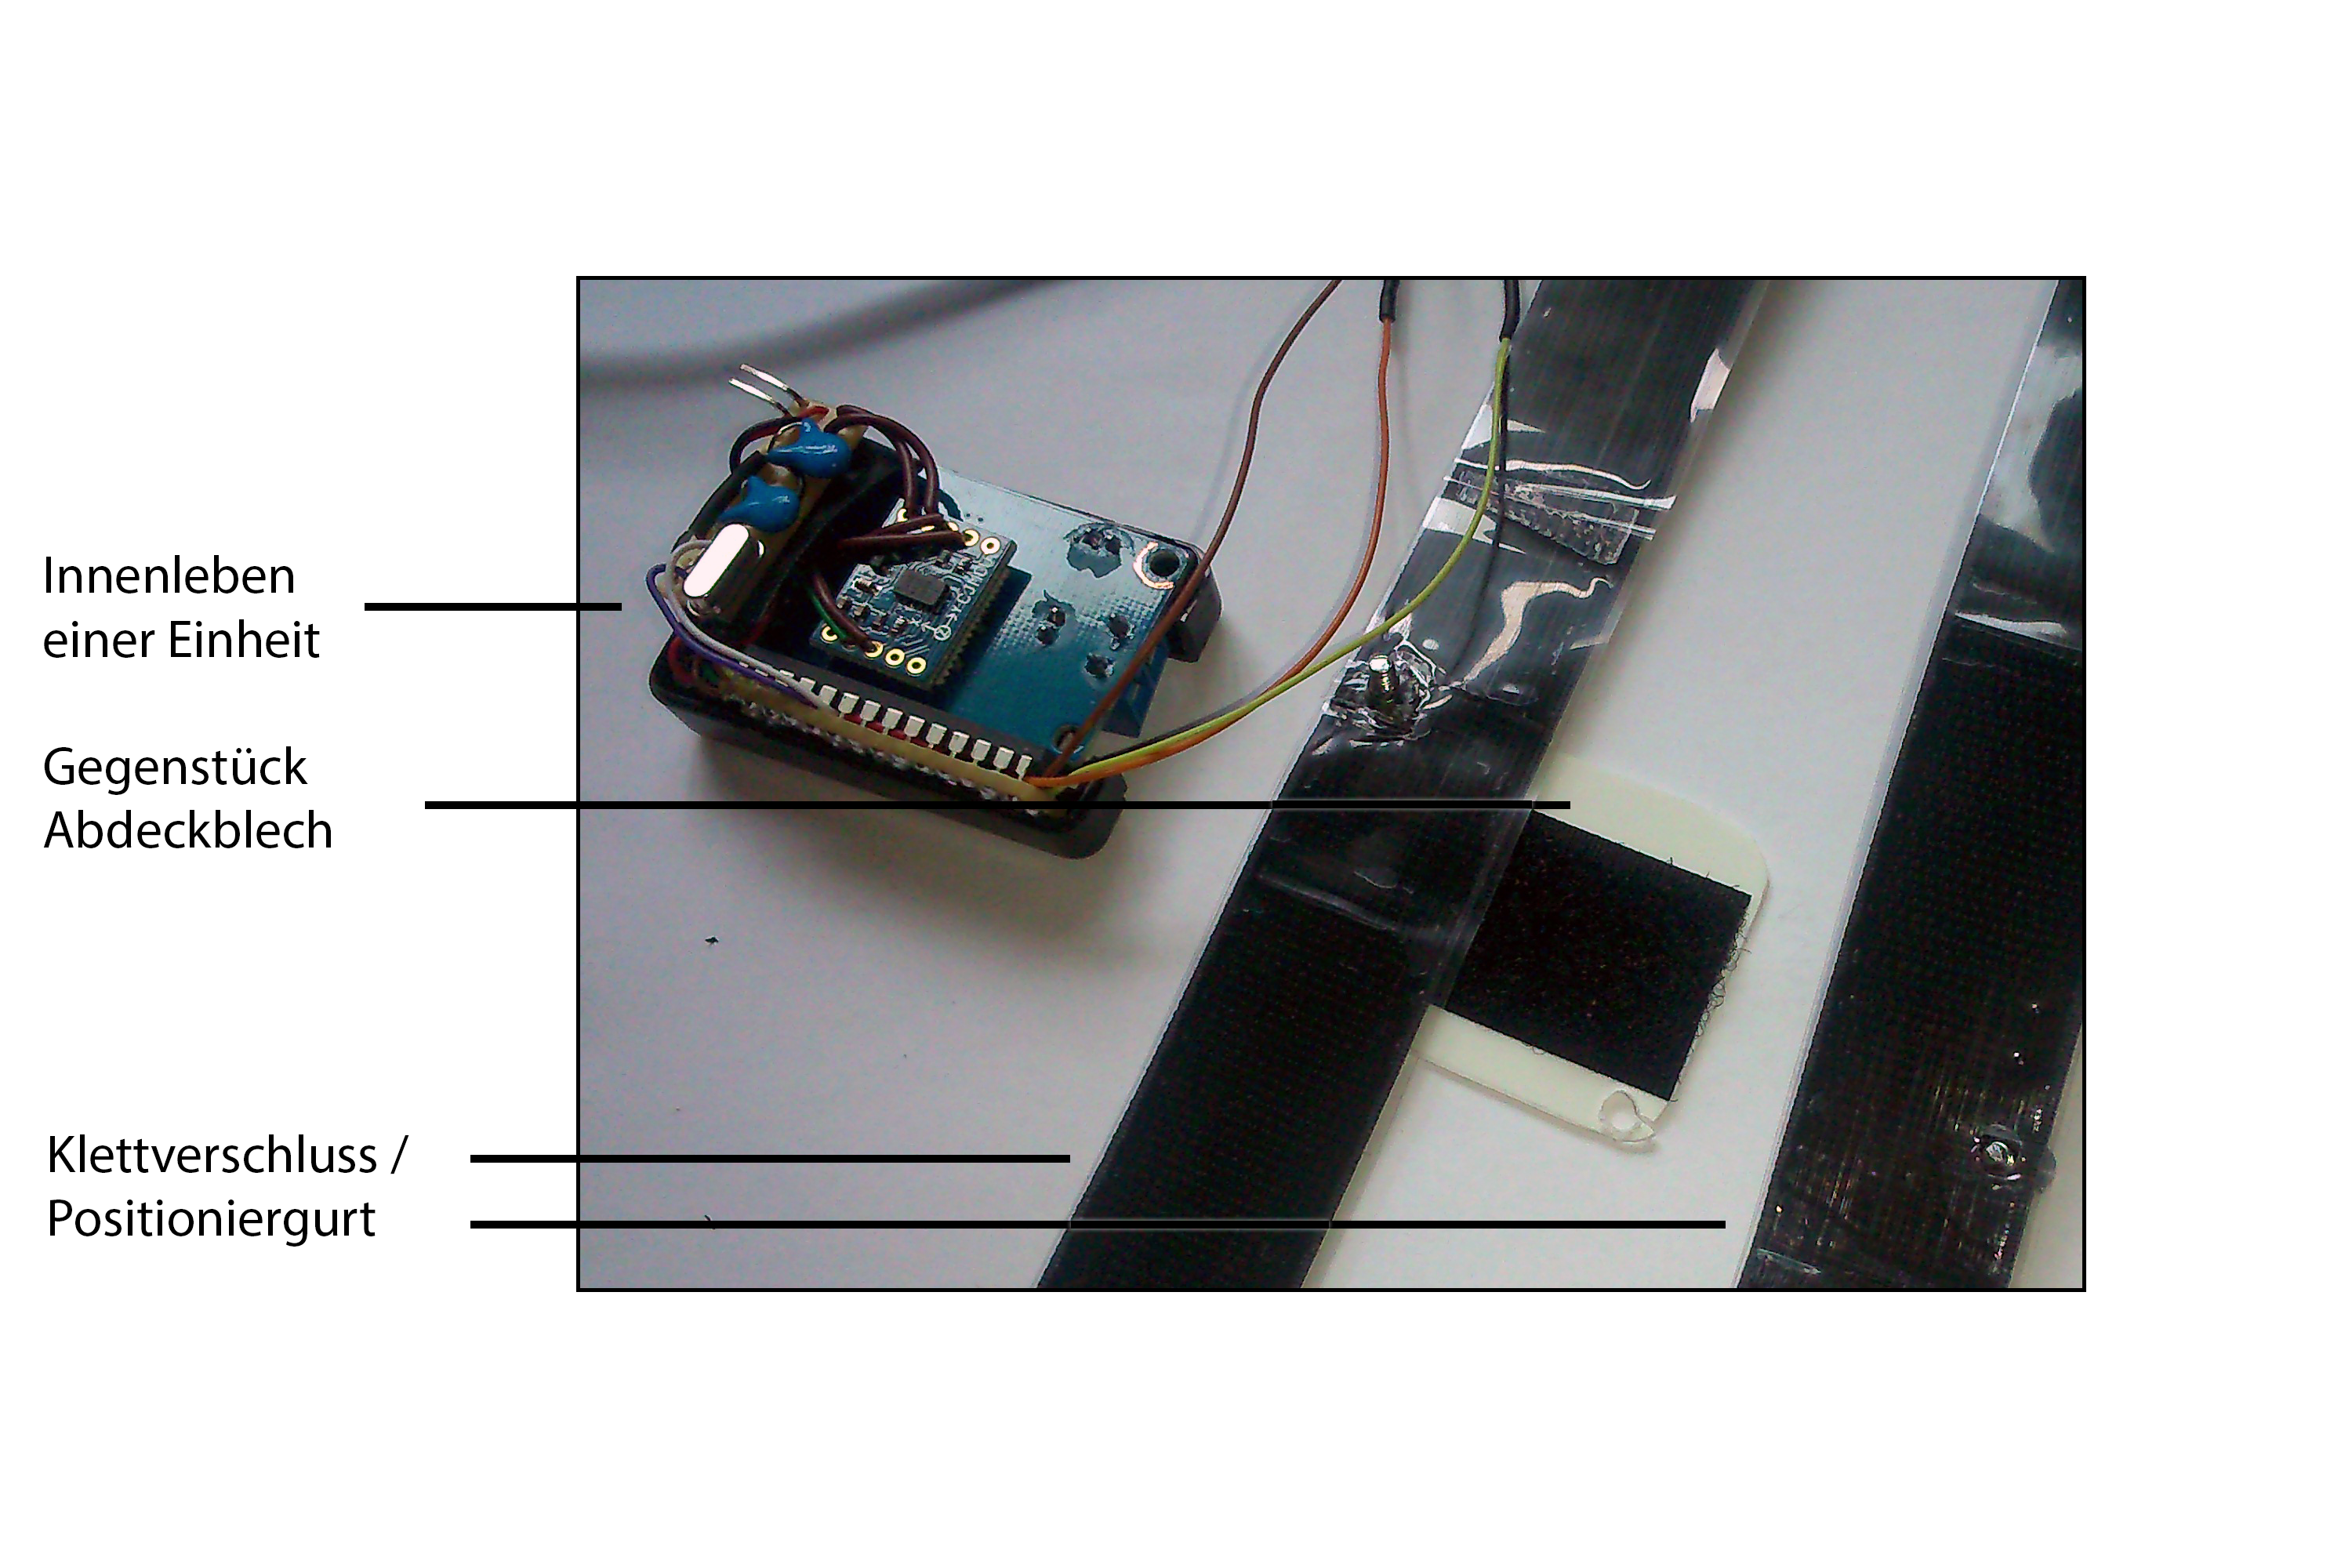
\includegraphics[width=1.0\linewidth]{03_Grafiken/Messsystem/McpExecutor2515Klettverschluss}
	\caption[Betaversion einer Mcp-Executor-Einheit - Klettverschluss]{Betaversion einer Mcp-Executor-Einheit - Klettverschluss}
	\label{fig:McpExecutorBetaKlettverschluss}
\end{figure}




\subsection{Release version}
\label{kap:McpExecutorReleaseversion}
Bei der Realease-Version der Mcp-Executor-Einheit wird die Beta-Version zun�chst bewertet und alle negativen Aspekte aufgezeigt und m�gliche L�sungen erarbeitet. Die zu verbessernden Punkte sind in Tabelle \ref{tab:McpExecutorEinheitNegAspekte} aufgelistet:

 
%\begin{figure}[H]
%	\centering
%	\includegraphics[width=0.7\linewidth]{03_Grafiken/Messsystem/McpExecutorRelease}
%	\caption[Release-Version einer Mcp-Executor-Einheit]{Release-Version einer Mcp-Executor-Einheit}
%	\label{fig:McpExecutorRelease}
%\end{figure}
\subsection{Programmaufbau}
\label{kap:McpExecutorProgrammaufbau}
\begin{enumerate}
	%
	% Setup-Routine
	%
	\item \textbf{Setup-Routine}\\
	% LISTING F�R SETUP() 
	Das Programm, welches auf der \gls{MCU} einer Einheit aktiv ist besteht aus einer Setup- und einer Loop-Routine. Innerhalb des Setups efolgt die Definition verschiedener Variablen und die Konfiguration der SPI-Schnisttstelle, sowie der Komponenten Adxl345 und Mcp2515 (s. Listing \ref{lst:mcpExecutorSetup}).
	In den Zeilen 4-6 und 8-10 werden die Ausg�nge zum Ausw�hlen der Ger�te, entsprechend der SPI-Schnittstelle, gesetzt. Dabei ist zu beachten, dass bei der Atmega-\gls{MCU} der Ausgang an Pin 10 immer immer gesetzt werden muss, auch wenn ein anderer Pin als Device-Selector verwendet wird. Der SIgnalzustand der Pins muss HIGH entsprechen, da bei einem Low-Pegel das entsprechende Ger�t ausgew�hlt wird.\\
	Zeile 12-13 initialisiert die SPI-Schnittstelle mit 5 Mhz und dem SPI-Mode 3 (CPOL = 1, CPHA = 1). Diese einzig verf�gbare Einstellung richtet sich nach dem Beschleunigungssensor Adxl345. Mit dem Aufruf der Routine SPI.begin() beginnt die Verwendung der Schnittstelle, sodass in den Zeilen 15-16 die Initialisierungsdaten an die Ger�te gesendet werden k�nnen. Diese beinhalten f�r den Sensor Adxl345 u.A. das Datenformat und f�r den Mcp2515 das CAN-Bus Setup. F�r das CAN-Bus Setup ist zu beachten, dass die Nachrichten jedes Teilnehmers einen spzifischen Identifier aufweisen muss.\\
	\label{lst:mcpExecutorSetup}
\begin{lstlisting}[language=Java, caption=Setup Routine]
void setup()
{
...
pinMode(CS_PIN_ADXL, OUTPUT);
pinMode(CS_PIN_MCP2515, OUTPUT);
pinMode(10, OUTPUT);

digitalWrite(CS_PIN_ADXL, HIGH);
digitalWrite(CS_PIN_MCP2515, HIGH);
digitalWrite(10, HIGH);

SPI.beginTransaction(SPISettings(5000000, MSBFIRST, SPI_MODE3));
SPI.begin();

initAdxl();
initMcp2515();
}
\end{lstlisting}
	%
	% Loop-Routine
	%
	\item \textbf{Loop-Routine}\\
	In der Loop-Routine (s. Listing \ref{lst:mcpExecutorLoop}) werden zwei Methoden aufgerufen, von denen die Prozedur \textit{getAdxlData()} die Sensordaten lie�t und zusammen mit einem Zeitstempel in ein Array speichert.
	Die Routine \textit{mcp2515\_load\_tx\_buffer()} schreibt die Daten nacheinander in die Sende-Buffer 1-3.\\
	Innerhalb der Routine \textit{getAdxlData()} erfolgt in Zeile 10 das Setzen der entsprechenden Registerwerte, um die Sensordaten auslesen zu k�nnen. In den Zeilen 12-15 erfolgt das Auslesen, indem der Selektor-Pin auf Low-Level gelegt wird. Anschlie�end erfolgt das Senden von 0-Werten, um per SPI die Sensordaten auszulesen (f�r jede Achse zwei Byte). In Zeile 17 wird noch die ID f�r das Ger�t angegeben.\\
	Innerhalb der Routine mcp2515\_load\_tx\_buffer0() erfolgt in den Zeilen 25-47 das Setzen der Registeradresse eines Sendebuffers, in Abh�ngigkeit welcher zuletzt genutzt wurde. In Zeile 51 werden in den ausgew�hlten Sendebuffer die Sensordaten gelegt und mit dem in Zeile 53 angegebenen Kommando auf den CAN-Bus geschickt.
	\label{lst:mcpExecutorLoop}
\begin{lstlisting}[language=Java, caption=Loop Routine]
void loop()
{
	getAdxlData();
	
	for (size_t i = 0; i < MESSAGE_SIZE_ADXL; i++) mcp2515_load_tx_buffer(ReadBuf[i], i, MESSAGE_SIZE_ADXL);
}
...
bool getAdxlData() {

	byte RegAddrBuf[] = { REGISTER_ACCEL_REG_X | REGISTER_ACCEL_SPI_RW_BIT | REGISTER_ACCEL_SPI_MB_BIT };
	
	setCsPin(CS_PIN_ADXL, LOW);
	SPI.transfer(RegAddrBuf[0]);
	for (int i = 0; i < 6; i++) ReadBuf[i] = SPI.transfer(0x00); 
	setCsPin(CS_PIN_ADXL, HIGH);
	
	ReadBuf[6] = EXECUTOR_ID;
	
	return true;
}
...
void mcp2515_load_tx_buffer(byte messageData, int byteNumber, int messageSize) {
	byte registerAddress;
	
	if (currentTxBuffer[0])
	{
	registerAddress = REGISTER_TXB0Dx[byteNumber];
	if (byteNumber == (messageSize-1))
	{
	currentTxBuffer[0] = false;
	currentTxBuffer[1] = true;
	}
	}
	else if (currentTxBuffer[1]) {
	registerAddress = REGISTER_TXB1Dx[byteNumber];
	if (byteNumber == (messageSize - 1))
	{
	currentTxBuffer[1] = false;
	currentTxBuffer[2] = true;
	}
	}
	else if (currentTxBuffer[2]) {
	registerAddress = REGISTER_TXB2Dx[byteNumber];
	if (byteNumber == (messageSize - 1))
	{
	currentTxBuffer[2] = false;
	currentTxBuffer[0] = true;
	}
	}
	
	mcp2515_execute_write_command(registerAddress, messageData, CS_PIN_MCP2515);
	
	for (int i = 0; i < 3; i++) if(currentTxBuffer[i] == true) mcp2515_execute_rts_command(i);	
}
\end{lstlisting}

\end{enumerate}
